\subheading{Wherein a Function To Fake the\\ Model Data is Written and Tested}
\section*{Section One and Two}

Before starting on identifying the system a good test is to produce a perfect
model based off made up parameters and see if the identifier is capable of
determining these parameters.  Following from this the first step was to create
a Matlab function that could take in the $C$ and $\beta$ parameters that defined
the system along with a frequency to evaluate it at ($\omega$) and a time to
evaluate it for ($t_\text{end}$).  This function is simply Equation
\ref{y_model} evaluated at the specified $C$, $\beta$ and $\omega$ with $t$
ranging from $0$--$t_\text{end}$ at a frequency of $1$ kHz.

To test the model function another model function utilising Matlab's in-built
\texttt{lsim} function was produced.  This uses the transfer function from
Equation \ref{transfer-function} along with the input from Equation
\ref{proportional-controller} to calculate the output.

Both models created were then plotted together with input values $C = 5$, $\beta
= 1$, $K_p = 60$, $f = 1.8$ and $t_\text{end} = 3$.  This can be seen in Fig.
\ref{section-two}.  Looking at this we can see that the steady state response of
the two systems is tending to be the same.  The major difference is in the
initial response, this is because the model used in the first equation is purely
a steady state model whereas the transfer function based model does base its
output off the initial conditions.

\begin{figure}
  \centering
  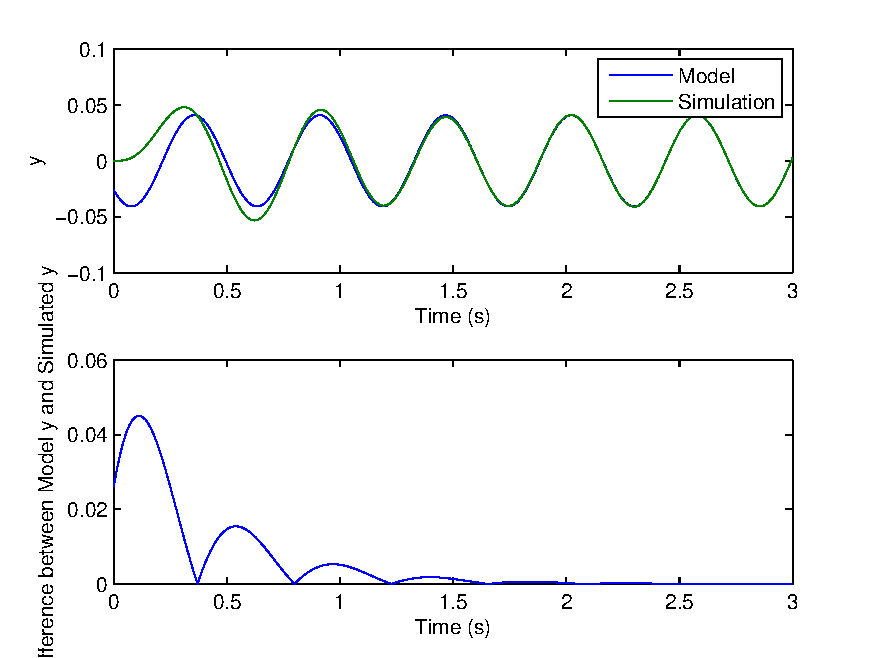
\includegraphics{images/section-two}
  \caption{Model vs Matlabs simulated values\label{section-two}}
\end{figure}
